\chapter{積分の応用}\label{chapt:integ_app}

積分は, 様々なことに応用される。2つの量の間の関係を知りたいとき, 
2つの量の微小量どうしの関係がわかれば, あとは積分で何とかなる。
本章ではその実例を学び, 積分がいかに便利で強力なツールかを
君に納得してもらう。

\section{円の面積}

ある図形の面積を知りたいとき, その図形を多くの小さな単純な図形に分解して, それぞれの
小図形の面積を足し合わせる(積分する)ことで, もとの図形の面積がわかる。例として, 
円の面積や球の体積の公式を導いてみよう。\mv

まず円の面積の公式を, 
オーソドックスなアプローチで求めてみよう。
\pref{sect:graph_integral}で学んだように, 関数のグラフが$x$軸より上にあるときは, 
その関数の定積分は, その関数と$x$軸で囲まれた図形の面積になる。それを使うのだ。

\begin{exmpl}\label{exmpl:surface2volume_sphere0}
2次元平面上に, 原点を中心とする半径$R$の円を考え, その面積を$S$とする。
この円が, $0\leq x$かつ$0\leq y$の範囲, つまり第一象限の範囲で, 
$x$軸と$y$軸とで囲む領域(つまり円板の1/4)の面積を求めてみよう。この円周の上の点$(x, y)$は,
\begin{eqnarray}x^2+y^2=R^2\end{eqnarray} 
を満たすが, 特にこの範囲では, 
\begin{eqnarray}y=\sqrt{R^2-x^2}\label{eq:circle_positive}\end{eqnarray} 
を満たす。
\begin{comment}
さて, この領域(円板の1/4)を, $y$軸に平行なたくさんの直線で切り刻もう。
すると, たくさんの細い帯ができる。幅$\Delta x$, 高さ$y$の帯の面積は, $y\Delta x$
である。さて, 帯を左から(原点に近い方から)順にならべて, それぞれの帯の右端の
位置を$x_1, x_2, \cdots, x_n$, 右端の高さを$y_1, y_2, \cdots, y_n$と
する(図\ref{fig:circlearea_strip})。$x_0=0$とする。明らかに, $\Delta x_k=x_k-x_{k-1}$
である。
\begin{figure}[h]
    \centering
    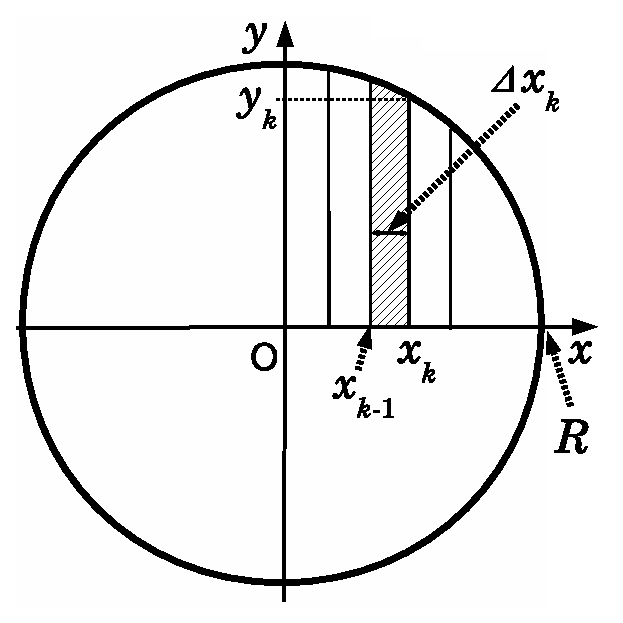
\includegraphics[width=5cm]{circlearea_strip.eps}
    \caption{円板を細長い帯で分割する。}\label{fig:circlearea_strip}
\end{figure}

この領域(円板の1/4)の面積$X$は, 
\begin{eqnarray}X\fallingdotseq \sum_{k=1}^{n}y_k \Delta x_k\end{eqnarray}
となる。この式を, \eref{eq:WhatIsIntegral15}と見比べながら, $n$を十分大きく, $\Delta x_k$を
十分小さくとれば, 次式のようになる:
\begin{eqnarray}X=\int_{0}^{R}y\,dx\label{eq:circlearea_strip_int0}\end{eqnarray}
ここで\eref{eq:circle_positive}を使えば, 次式のようになる:
\end{comment}
従って, この領域(円板の1/4)の面積$X$は, 次式のようになる:
\begin{eqnarray}X=\int_{0}^{R}\sqrt{R^2-x^2}\,dx\label{eq:circlearea_strip_int}\end{eqnarray}
\end{exmpl}

\begin{q}\label{q:int_circle1} \eref{eq:circlearea_strip_int}を使って, 
\begin{enumerate}
\item 次式を示せ:
\begin{eqnarray}X=\frac{\pi R^2}{4}\end{eqnarray}
\item それを使って次式を示せ。
\begin{eqnarray}S=\pi R^2\label{eq:circlearea}\end{eqnarray}
\end{enumerate}\end{q}
\mv

このアプローチは, \fref{fig:integral_strip}のように, 図形を縦長の
短冊に分割するという作戦だ。ところが, 円は四方八方に丸いので, もっと
エレガントに求まるのだ:

\begin{exmpl}\label{exmpl:surface_circle0} 半径$R$の円板を, 
小さな幅の円環の集まりと考える(\fref{fig:circlearea_ring})。
すなわち, 円を$n$個の同心円で分割し, 
小さい円から順に, それぞれ半径$r_1, r_2, \cdots, r_n$とする。
$r_0=0$とし, $r_n=R$とする。$k$を1以上$n$以下の整数とし, 
半径$r_{k-1}$の円と半径$r_k$の円で挟まれた円環を考えよう。
その幅を$\Delta r_k$とする。つまり$\Delta r_k=r_k-r_{k-1}$である。
$\Delta r_k$が十分に小さいなら, この円環の面積$\Delta S_k$は, 
\begin{eqnarray} 
\Delta S_k\fallingdotseq 2\pi r_k\,\Delta r_k
\end{eqnarray}
となる(円周の長さと幅の積\footnote{
厳密に言えば, 円環の面積を求めるには円環の外縁と内縁の中間に
位置する円の半径を使わねばならないが, 幅$\Delta r_k$が十分に小さければ, 
これは外縁の円の半径や内縁の円の半径にほぼ一致する。})。
すると, 円の面積$S$は, $\Delta S_k$を足しあわせたものにほぼ等しい:
\begin{figure}[h]
    \centering
    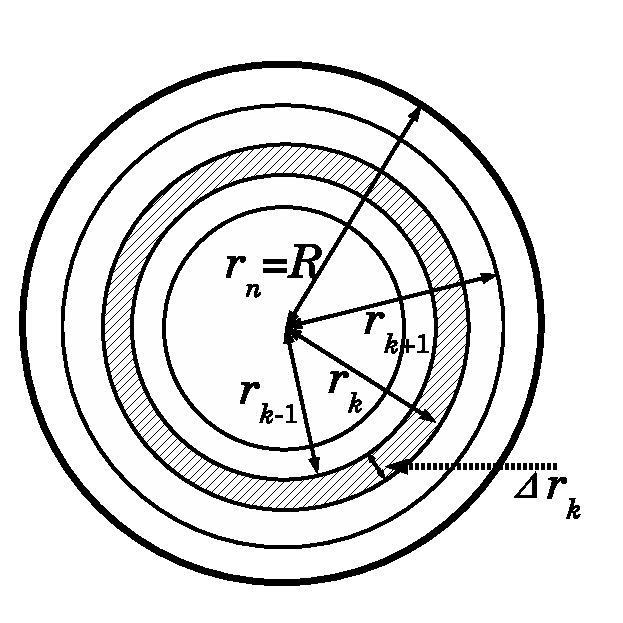
\includegraphics[width=5cm]{circlearea_ring.eps}
    \caption{円板を細い円環で分割する。}\label{fig:circlearea_ring}
\end{figure}
\begin{eqnarray}
S\fallingdotseq \sum_{k=1}^{n}\Delta S_k=\sum_{k=1}^{n}2\pi r_k \Delta r_k
\end{eqnarray}
となる。この式を, \peref{eq:WhatIsIntegral15}と見比べながら, $n$を十分大きく, $\Delta r_k$を
十分小さくとれば, 次式になる:
\begin{eqnarray}
S=\int_{0}^{R}2\pi r\,dr=[\pi r^2]_0^R=\pi R^2\label{eq:circlearea_ring_int}
\end{eqnarray}
この積分は, \eref{eq:circlearea_strip_int}の積分よりも
ずっと簡単だ。なお, こういう考え方を, とある高校の先生は
「バウムクーヘン積分」と教えているらしい。なんかイメージわかるよね。(例おわり)
\end{exmpl}\mv

\begin{q}\label{q:int_circle0} 例\ref{exmpl:surface_circle0}の
やり方を再現して, 円の面積の公式を導け。適当に省略・簡略化し, 
簡潔かつ論理的にまとめ直せ。\end{q}

\begin{comment}
\begin{q}\label{q:int_circle2} 円の面積の公\eref{eq:circlearea}を, さらに別のアプローチで
考えてみよう。半径$R$の円板を, 微小な頂角$\Delta \theta$の扇形に分割して考えて
(図\ref{fig:circlearea_angle}), \eref{eq:circlearea}を導け。
ヒント: 微小な頂角$\Delta \theta$の扇形はほとんど三角形とみなすことができる。
その底辺の長さはほとんど弧の長さに等しく, $R\Delta \theta$であり, 高さは
ほとんど半径に等しく, $R$である。
\begin{figure}[h]
    \centering
    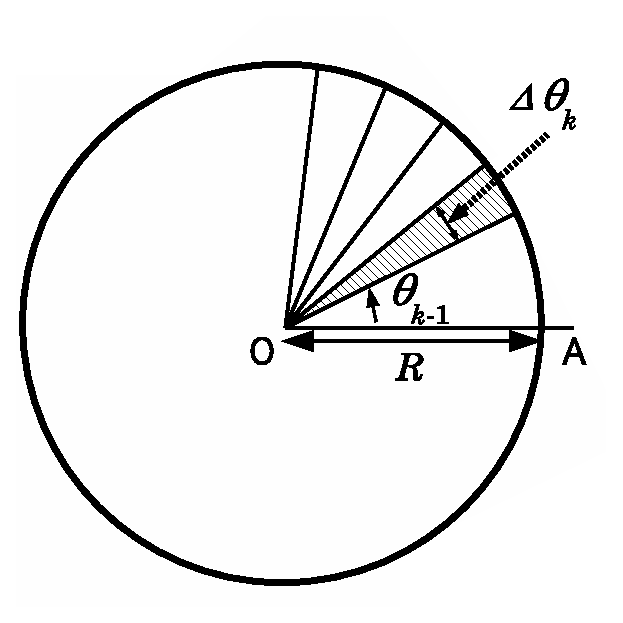
\includegraphics[width=5cm]{circlearea_angle.eps}
    \caption{円板を細い扇形で分割する。円の中心を通る直線OAを基準線とし, そこから角$\theta_k$
にある半径で円を分割する($k=0, 1, 2, \cdots, n$)。$\theta_0=0, \theta_n=2\pi$とする。
角$\theta_{k-1}$と角$\theta_k$で挟まれた部分は, 頂角$\Delta \theta_k
=\theta_k-\theta_{k-1}$の扇形になる。}\label{fig:circlearea_angle}
\end{figure}
\end{q}\mv

\noindent{\textbf{答}}\ref{q:int_circle2} 略解: 
\begin{eqnarray}
S=\int_{0}^{2\pi}\frac{R^2\,d \theta}{2}=\pi R^2
\end{eqnarray}
\end{comment}

\section{球の体積}

次は球の体積の公式を求めてみよう。

\begin{exmpl}\label{exmpl:volume_sphere0}
3次元空間中に$x$, $y$, $z$の各軸を考え, 原点を中心とする半径$R$の球を考える。
その体積を$V$とする。$-R\leq x \leq R$の区間を$-R=x_0<x_1<\cdots<x_n=R$となる
ように$x_0, x_1, \cdots, x_n$という点で分割し, 各点を通り$x$軸に垂直な平面
で球を刻む。すると, $x=x_k$での切り口は, 半径が$\sqrt{R^2-x_k^2}$の円になる。
さて, $x_{k-1}$と$x_k$が十分に近ければ, $x=x_{k-1}$での切り口と$x=x_{k}$での
切り口は, ほぼ同じ大きさの円とみなせるので, それらで挟まれた円盤(薄い円柱)
の体積$\Delta V_k$は, 
\begin{eqnarray}
\Delta V_k=\pi\bigl(\sqrt{R^2-x_k^2}\,\bigr)^2\Delta x_k=\pi(R^2-x_k^2)\Delta x_k\quad\quad\quad
\label{eq:volume_sphere02}
\end{eqnarray}
となる(底面積×高さ)。このような円盤を全ての$k$について考えて足し合わせれば, 
球が再現される。従って, その体積は, 
\begin{eqnarray}
V&=&\lim_{\substack{n\rightarrow \infty\\\Delta x_k\rightarrow 0}}\sum^{n}_{k=1}\pi(R^2-x_k^2)\Delta x_k\label{eq:volume_sphere04}\\
 &=&\int_{-R}^{R}\pi(R^2-x^2)\,dx=\cdots=\frac{4\pi R^3}{3}\label{eq:volume_sphere06}
\end{eqnarray}
(例おわり)
\end{exmpl}


\begin{freqmiss}{\small\textgt{\eref{eq:volume_sphere06}で, 
\begin{eqnarray*}
=\int_{-R}^{R}\pi(R^2-x_k^2)\,dx=\cdots
\end{eqnarray*}
と書いてしまう} ... $x_k$の$k$を残してはダメです。$\sum$が$\int$に
なった瞬間, $x_k$の$k$は消えるのです。$x_k$と$x_{k+1}$の間隔が
限りなく0に近づき, $k$という「背番号」が意味を失うからです。}\end{freqmiss}

\begin{q}\label{q:int_ball2} 例\ref{exmpl:volume_sphere0}
を再現し, 球の体積の公式を導け。丸写しにするのでなく, 
教育的な説明は省略して, 自分なりに簡潔に書くこと。\end{q}\mv

ところで, 有限の微小量, つまり「$\Delta$なんとか」で考えるのは
めんどくさい。毎回毎回, 結局は$\Delta$が$d$になって$\sum$が$\int$
になって添字の$k$が消えるのだ。そこで, これらの議論は, 
いきなり無限小($dx$とか$dV$とか)を使って簡略的に書くことにしよう。
\begin{exmpl} (例\ref{exmpl:volume_sphere0}の書き直し)\\
3次元空間中に$x$, $y$, $z$の各軸を考え, 原点を中心とする半径$R$の球を考える。
その体積を$V$とする。球を, $x$軸に垂直で厚み$dx$の円盤の集まりとみなす。
各円盤の半径は$\sqrt{R^2-x^2}$なので, その体積$dV$は, 次式になる:
\begin{eqnarray}
dV=\pi(\sqrt{R^2-x^2})^2dx=\pi(R^2-x^2)dx\label{eq:volume_sphere02d}
\end{eqnarray}
これを積分して, 
\begin{eqnarray}
V=\int_{-R}^{R}\pi(R^2-x^2)\,dx=\cdots=\frac{4\pi R^3}{3}\label{eq:volume_sphere06d}
\end{eqnarray}
(例おわり)
\end{exmpl}

さて, この球の体積の公式($\frac{4\pi R^3}{3}$)は記憶せよ。
語呂合わせは, 「身の上に心配あるので参上」という。
つまり, 「3(身)の上に$4\pi r$(心配ある)ので3乗(参上)」

ところで, 例\ref{exmpl:volume_sphere0}は, 例\ref{exmpl:surface2volume_sphere0}
によく似た発想である。例\ref{exmpl:surface2volume_sphere0}では円を多くの狭い
長方形で平行に刻んだが, ここでは球を多くの狭い円盤で平行に刻んだのだ。

一方, 円を同心円で刻んだ例\ref{exmpl:surface_circle0}のような
発想でも球の体積は求まるのではないだろうか? やってみよう! 
まず, 半径$r$の球の表面積が$4\pi r^2$であるのは既知とする。

\begin{exmpl}\label{exmpl:volume_sphere2} 半径$R$の球(体積を$V$とする)
を, 小さな幅の球殻の集まりと考える。半径$r$, 厚さ$dr$の球殻の
体積$dV$は, 半径$r$の球面積と球殻の厚さの積, つまり
\begin{eqnarray}
dV=4\pi r^2dr\label{eq:volume_sphere3}
\end{eqnarray}
となる。これを積分して, 
\begin{eqnarray}
V=\int_{0}^{R}4\pi r^2\,dr=\Bigl[\frac{4\pi r^3}{3}\Bigr]_0^R
=\frac{4\pi R^3}{3}\label{eq:volume_sphere4}
\end{eqnarray}
(例おわり)
\end{exmpl}\mv

\begin{q}\label{q:int_ball3} 例\ref{exmpl:volume_sphere2}
を再現して, 球の体積の公式を導け。\end{q}
\mv


ここで, 面白いことに気付く。: 半径$r$を変数にとると, 円の周長と面積の
関係や, 球の表面積と体積の関係は, 一方が他方の微分(積分)となって
いるのだ(図\ref{fig:circle_ball_biseki})。
\begin{figure}[h]
    \centering
    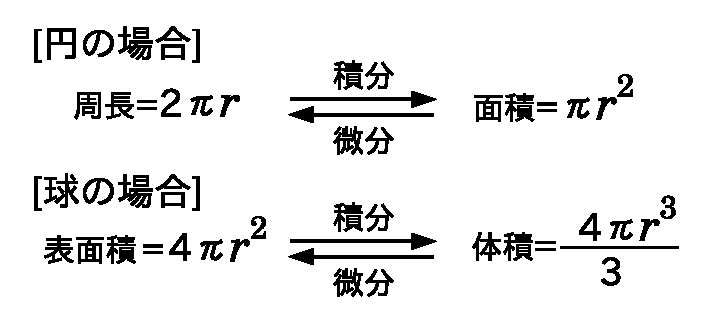
\includegraphics[width=6cm]{circle_ball_biseki.eps}
    \caption{円の周長と面積, 球の表面積と体積には, 微分積分の関係がある。
半径で微分すると「長さ」の次元がひとつ減り, 半径で積分すると
「長さ」の次元がひとつ増えることにも注意しよう。}\label{fig:circle_ball_biseki}
\end{figure}

なぜだろう? 例えば\eref{eq:volume_sphere3}を見てみよう。この両辺を$dr$
で割れば, $dV/dr=4\pi r^2$が出てくるではないか!

これらを手がかりにすれば, 球の体積や表面積の公式を思い出すことができる
(\pref{q:sphere_SV_dimcheck}の問\ref{q:sphere_SV_dimcheck}
も参照せよ)。公式は, いろんな観点から体系的に理解することが大事なのだ。

\begin{faq}{\small\textgt{例\ref{exmpl:surface_circle0}では
円の周長の公式($2\pi r$)を, 例\ref{exmpl:volume_sphere2}では
球の表面積の公式($4\pi r^2$)を, それぞれ既知として使いましたが, 
そもそもそれらはどうやって導出されるのですか?} ... 
良いところに気づきました。円の周長の公式($2\pi r$)は, ラジアンの定義
と, 平面図形の相似性(相似比に応じて長さも変わる)から出てきます。
球の表面積の公式($4\pi r^2$)は, 実は球の体積の公式を微分して
導くのです。つまり, 例\ref{exmpl:volume_sphere0}で体積を求めて, 
それを半径で微分して表面積の公式を導くのです。つまり, 例\ref{exmpl:volume_sphere2}
を逆に辿るのが, 本来の考え方です。}\end{faq}
\mv
\begin{comment}
また, 球は, 球をすっぽり包む立方体(1辺の長さ$2r$)よりも小さいので, 球の体積は, 
その立方体の体積, つまり$(2r)^3=8r^3$より小さいはず。従って, もし公式を忘れかけて, 
$r^3$の係数が$4\pi/3$なのか$4\pi$なのか自信なくなっても, 
$r^3$の係数は$8$以上になることは絶対にないから, $4\pi=12.5\cdots$になるわけがない! 
と判断できる。\hv

\begin{q}\label{q:int_ball0} \eref{eq:ballvolume}を利用して, 
半径$r$の球の表面積$S(r)$が次式であることを示せ。
\begin{eqnarray}
S(r)=4\pi r^2\label{eq:ballsurface}
\end{eqnarray}
\end{q}\mv
\end{comment}


%ところで, おもしろい事実がある。球の表面積は, それをすっぽり入れてしまう円筒の側面積
%(ふたと底を除いた表面積)と同じなのだ。
%(図\ref{fig:sphere_pipe})
%実際, 円筒は, 高さが$2r$, 一周が$2\pi r$なので, その側面積は, 
%$2r\times2\pi r=4\pi r^2$となり, 球の表面積と一致する。これはアルキメデスが
%発見した。喜んだアルキメデスは, この定理を示す球と円筒の絵を, 自分の墓標に刻む
%ように遺言したらしい。
%\begin{figure}[h]
%    \centering
%    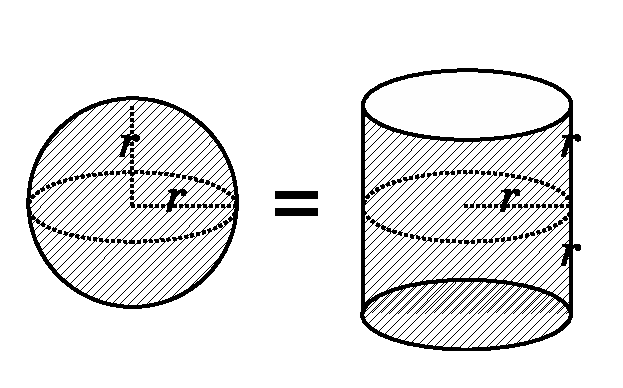
\includegraphics[width=7cm]{sphere_pipe.eps}
%    \caption{半径$r$の球の表面積と, 半径$r$, 高さ$2r$の円筒の側面積は, 
%どちらも$4\pi r^2$で等しい。}\label{fig:sphere_pipe}
%\end{figure}

%\begin{q}\label{q:int_circle_ball_diff} \
%\begin{enumerate}
%\item \eref{eq:circlearea}を$R$で微分すると円周の長さの公式が得られることを確認せよ。
%\item なぜそうなるのか, 説明せよ。
%\item \eref{eq:ballvolume}を$R$で微分すると球の表面積の公式が得られることを確認せよ。
%\item なぜそうなるのか, 説明せよ。
%\item 球の体積の\eref{eq:ballvolume}を, 半径$r$のかわりに直径$w$を使って書き直せ。
%\item それを$w$で微分すると, 球の表面積の公式にはならないことを確認せよ。
%\item それはなぜなのか, 説明せよ。
%\end{enumerate}\end{q}


\begin{faq}{\small\textgt{∫は積分, $d$は微分を表すなら,∫$d$○=○ですか?}
... ざっくり言えばそうです。∫は$\Sigma$の極限で, $d$は微小な差を表します。
○の細かい差をぜんぶ集めたら○自身になります。りんごをこまかく切り刻んで
よせあつめたら, りんごになります。

\textgt{りんごをこまかく切り刻んでよせあつめてもりんごにならないと思います}
... たしかに, 汁が出てぐちゃぐちゃになりそうだもんね。}\end{faq}




\section{速度・加速度}

微分を使って学んだ速度と加速度(P.\pageref{secvelocity_and_acceleration})を, 
積分を使って振り返ろう。その前にひとつ準備をする。\eref{eq:fb_fa_int_f'}を
思い出そう。任意の関数$f(x)$について, 
\begin{eqnarray}
f(x_0+\Delta x)=f(x_0)+\int_{x_0}^{x_0+\Delta x}f'(x)\,dx\label{eq:fb_fa_int_f'_again}
\end{eqnarray}
だった。この式で, $x$を$t$に, $x_0$を$t_0$に, $x+\Delta x$を$t_1$に形式的に置き換えると, 
\begin{eqnarray}
f(t_1)=f(t_0)+\int_{t_0}^{t_1}f'(t)\,dt\label{eq:fb_fa_int_f'_again_t}
\end{eqnarray}
となる。これで準備OK。

さて, ある点Pが$x$軸上を運動しており, 時刻$t$で位置$x(t)$, 速度$v(t)$, 加速度$a(t)$であるとき, 
\begin{eqnarray}
\frac{dx}{dt}=v(t)\label{eq:dxdt_v}\\
\frac{dv}{dt}=a(t)\label{eq:dvdt_a}
\end{eqnarray}
だった(速度と加速度の定義)。ここで, \eref{eq:dxdt_v}より, $x'(t)=v(t)$ということを
頭に置いて, \eref{eq:fb_fa_int_f'_again_t}を$x(t)$に適用すると(つまり$f$を$x$に
形式的に置き換えると), 
\begin{eqnarray}
x(t_1)=x(t_0)+\int_{t_0}^{t_1}v(t)\, dt\label{eq:x1_x0_intv}
\end{eqnarray}
となる。これは時刻$t_1$での位置を, 時刻$t_0$での位置と, $t_0$から$t_1$までの
間の速度の積分で表す式である。同様に, \eref{eq:dvdt_a}より, $v'(t)=a(t)$ということを
頭に置いて, \eref{eq:fb_fa_int_f'_again_t}を$v(t)$に適用すると, 次式になる:
\begin{eqnarray}
v(t_1)=v(t_0)+\int_{t_0}^{t_1}a(t)\, dt\label{eq:v1_v0_inta}
\end{eqnarray}

\begin{q}\label{q:x_v_dif_int} \eref{eq:x1_x0_intv}から\peref{eq:xtdtxtvtdt}を導け。\end{q}

\begin{q}\label{q:v_a_dif_int} \eref{eq:v1_v0_inta}から\peref{eq:vtdtvtatdt}を導け。\end{q}
\mv

さて, \textgt{もし, 加速度$a$が時間によらず一定であれば}, 
\eref{eq:v1_v0_inta}の定積分(定数関数の定積分, チョー簡単!)より, 
\begin{eqnarray}v(t_1)=v(t_0)+a(t_1-t_0)\end{eqnarray}
となる。$t_0=0$とし, $t_1$を改めて$t$と書き直せば, 
\begin{eqnarray}v(t)=v(0)+at\label{eq:v_v0_at}\end{eqnarray}
となる。これを\eref{eq:x1_x0_intv}に代入すれば, 
\begin{eqnarray}
x(t_1)&=&x(0)+\int_{0}^{t_1}\{v(0)+at\}\, dt\nonumber\\
      &=&x(0)+v(0)t_1+\frac{1}{2}at_1^2\label{eq:x_x0_va0}
\end{eqnarray}
となる。再び$t_1$を改めて$t$と書き直せば,
\begin{eqnarray}x(t)=x(0)+v(0)t+\frac{1}{2}at^2\label{eq:x_x0_va}\end{eqnarray}
となる。

\eref{eq:v_v0_at}と\eref{eq:x_x0_va}は, 高校理科(物理)で習う
式である。これを一生懸命に記憶した人もいるだろうが, この式の実体は
定数関数$a$を時刻で2回積分しただけである。その仕組みを知ってしまえば, 
わざわざ覚えるようなものではないことがわかるだろう。

さて, 注意してほしいのは, これらは\textgt{一定の加速度の運動(等加速度直線運動)
でしか成り立たない!}ということ。というのも, 
\eref{eq:v1_v0_inta}が\eref{eq:v_v0_at}になるのは, $a$が定数だからだし, 
\eref{eq:x_x0_va0}の積分がこうなるのも$a$が定数だからだ。
もし$a$が定数でない, つまり加速度$a$が時間的に変化するなら, 
これらは成り立たない。そういうときは\eref{eq:x1_x0_intv}と\eref{eq:v1_v0_inta}
に戻るしかない。しかしそういう「使用上の注意」も, この式の数学的な由来を
理解していれば, 覚えるまでもない, アタリマエのことだ。

\begin{faq}{\small\textgt{高校ではなぜそう教えない
のでしょう?} ... わかりません。高校物理の「公式」のほとんどは, 
こんなかんじで, 何かの法則やシンプルな仮定から, 数学的に導出
できます。多くの高校生は, 物理は公式が多くて嫌と言いますが, 
真実は反対で, 物理の本質的な公式は少しだけです。}\end{faq}
\mv

\begin{comment}
\section{仕事}\index{しごと@仕事}

中学理科では, 仕事は「力と, その力が働く点が"力と同じ向き"に動いた距離との掛け算」
であると習ったが, それが意味を持つのは, その点の移動中に, 
力が変化しないときだけだ(でなければ, どの時点での力を掛け
算すればいいのかわからない)。では, 移動中に力が変わる場合は, 
仕事はどう定義されるのだろう?

いま, $x$軸上で, ある物体に力$F(x)$が$x$軸に平行にかかっており, 
物体を$\Delta x$だけ動かす。力$F(x)$は位置$x$によって変わる
が, $\Delta x$は微小なため, その間は力はほとんど変化しないと
考える(というか, そう考えても構わないくらいに小さな$\Delta x$を考える)。
すると, その間にその力がする仕事$\Delta W$は, 中学の仕事の定義から, 
\begin{eqnarray}
\Delta W\fallingdotseq F(x)\Delta x \label{eq:work}
\end{eqnarray}
である。これをたくさん繰り返すことを考えよう。

位置$x=a$にある物体を, 位置$x=b$まで運ぶ。この区間を, $n$個の
小区間に分割し, それぞれの小区間の境目を$x_1, x_2, \cdots, x_{n-1}$
とし, $x_0=a$, $x_n=b$とする。

各小区間で\eref{eq:work}が成り立つと考える。すると, 位置$x_{k-1}$から
位置$x_k$までの小区間$\Delta x_k$の間の移動における仕事$\Delta W_k$は, 
\begin{eqnarray}
\Delta W_k\fallingdotseq F(x_k)\Delta x_k\label{eq:one_step_before_work1}
\end{eqnarray}
である。これを全区間で合計したものを, 物体を$x_0$から$x_n$まで
運ぶときの全体の仕事$W$とする:
\begin{eqnarray}
W= \sum_{k=1}^{n}\Delta W_k\fallingdotseq\sum_{k=1}^{n}F(x_k)\Delta x_k \label{eq:one_step_before_work2}
\end{eqnarray}
ここで$n$を十分大きくとって, $x_1, x_2, ..., x_n$の分割を十分に細かく
すれば, すなわち, \eref{eq:one_step_before_work2}の極限として, 
\begin{eqnarray}
W=\lim_{\substack{n\rightarrow \infty\\\Delta x_k\rightarrow 0}}\sum_{k=1}^{n}F(x_k)\Delta x_k
\end{eqnarray}
を考えれば, \peref{eq:WhatIsIntegral2}より, 次式が成り立つ:
\begin{itembox}{仕事の定義(力が一定でない場合)}
物体を位置$a$から位置$b$まで直線上を運ぶとき, 力$F(x)$がなす仕事は, 
\begin{eqnarray}
W=\int_{a}^{b} F(x)\,dx \label{eq:work2}
\end{eqnarray}
\end{itembox}
これは, 中学理科や高校物理では習わない, 一般性の高い「仕事の定義」
である\footnote{しかしこの定義は移動が$x$軸に限定されないとき
(曲線的な移動のとき)には無力である。そういうときは, 
ベクトルの内積を使う「線積分」という数学が必要。}。

\eref{eq:one_step_before_work1}〜\eref{eq:work2}は, 
有限の微小量$\Delta x$, $\Delta W$をいちいち使って書いたりせず, 
いきなり無限量($dx$, $dW$)を使って, 次のように簡略的に書いてもよい:

\begin{eqnarray}
dW=F(x)\,dx
\end{eqnarray}
両辺を積分して, 
\begin{eqnarray}
\int_0^W dW=\int_a^b F(x)\,dx
\end{eqnarray}
すなわち, 
\begin{eqnarray}
W=\int_a^b F(x)\,dx
\end{eqnarray}

%
\begin{q}\label{q:gas_work}
気体を膨張させたり圧縮したりするときの仕事を考えよう。ある気体が, 断面積$A$の
シリンダー(筒状の容器)に入っており, 上面がピストンで蓋してある。
鉛直上向きに$x$軸をとり, シリンダーの底面で$x=0$とする。ピストンは$x$軸にそって上下に
動くことができる。最初, ピストン(つまり蓋)は$x=h$にあって静止しているとする
(図\ref{fig:gas_piston})。
ピストンは十分に軽いとし, 重力を無視する。気体の圧力を$P$とする。
\begin{figure}[h]
    \centering
    \includegraphics[width=3.7cm]{gas_piston.eps}
    \caption{気体の入ったシリンダー。}\label{fig:gas_piston}
\end{figure}
\begin{enumerate}
\item 気体の体積$V$は, $V=Ah$と表せることを示せ。
\item 気体がピストンに及ぼす力$F_1$は次式のようになることを示せ:
\begin{eqnarray}F_1=PA\label{eq:gas_work1}\end{eqnarray}
\item 外部からピストンにかかる力(外力という\footnote{この外力が
具体的に何によるものかは, ケースバイケースであり, ある場合は誰かが手で押さえ
込んでいるのかもしれないし, ある場合はシリンダー外部に充満する気体
の圧力によるものかもしれない。この問題ではその詳細は気にしない。})
を$F_2$とすると, それは次式になることを示せ:
\begin{eqnarray}F_2=-PA\label{eq:gas_work2}\end{eqnarray}
\item 次に, ピストンをゆっくり動かして, $x=h+dh$の位置に移動させることを考えよう。
$dh>0$なら, 気体は膨張し, $dh<0$なら気体は圧縮される。$dh$は微小であり, 
ピストンが$x=h$から$x=h+dh$まで動く間に$F_1$や$F_2$はほとんど一定である
とみなす。このとき, 外力がなす仕事$dW$は, 
\begin{eqnarray}dW=F_2\,dh=-PA\,dh\label{eq:gas_work3}\end{eqnarray}
となることを示せ。
\item ピストンの移動後に気体の体積は$V+dV$になったとする($dV$は体積の変化)。次式を示せ:
\begin{eqnarray}dV=A\,dh\label{eq:gas_work4}\end{eqnarray}
\item \eref{eq:gas_work3}, \eref{eq:gas_work4}より次式を示せ:
\begin{eqnarray}dW=-P\,dV\label{eq:gas_work5}\end{eqnarray}
\item ピストンを大きく動かし, 体積が$V_1$から$V_2$になるまで変化させることを考えよう。
この間に外力がなす仕事$W$は次式のようになることを示せ:
\begin{eqnarray}
W=-\int_{V_1}^{V_2}P\,dV
\end{eqnarray}
\item ここで, 気体は理想気体であるとしよう。つまり, 理想気体の状態方程式:
\begin{eqnarray}PV=nRT\end{eqnarray}
が成り立つとする($n$はモル数, $R$は気体定数, $T$は絶対温度)。次式が成り立つことを示せ:
\begin{eqnarray}
W=-\int_{V_1}^{V_2}\frac{nRT}{V}\,dV
\end{eqnarray}
\item ここでさらに, ピストンの移動を十分にゆっくり行い, その過程では
\textgt{温度$T$は一定に維持する}と, 次式が成り立つことを示せ:
\begin{eqnarray}
W=nRT\ln\frac{V_1}{V_2}
\end{eqnarray}
\item 1モルの理想気体を摂氏0度(一定)で体積を半分まで圧縮するときに外力がなす仕事を求めよ。
\end{enumerate}
\end{q}
\mv

\eref{eq:gas_work5}は, 化学や熱力学で, 非常によく出てくる式である。ここでは外力が
なす仕事を考えたが, 気体(の圧力)がなす仕事$dW'$は, 
\begin{eqnarray}
dW'=P\,dV
\end{eqnarray}
となる(力の向きが逆なので仕事の符号も逆になる)。この式もよく使われる
\footnote{化学や熱力学では, 教科書によって, 外力のなす仕事を$dW$とするものと, 
気体がなす仕事(すなわちここで$dW'$とあらわしたもの)を$dW$とするものがあるので, 
気をつけよう。}。
\vv
\end{comment}




\section{微分方程式}\label{sect_diffeq0}

\pref{sect_diffeq_exp}で, 簡単な微分方程式を学んだ。そのとき, 
\begin{eqnarray}
f'(x)=af(x)\label{eq:diffeq0_again}
\end{eqnarray}
という微分方程式の解は
\begin{eqnarray}
f(x)=f(0)e^{ax}\label{eq:diffeq000_IC_again}
\end{eqnarray}
となることを\eref{eq:diffeq000_IC}で学んだ。\eref{eq:diffeq000_IC_again}が\eref{eq:diffeq0_again}
を満たすことは, 代入してみればすぐにわかる。しかし, ここでは, 
そういう天下りなやり方を使わないで微分方程式の解を
得る方法を学ぶ。\\

例えば, 関数$f(x)$について, 
\begin{eqnarray}f'(x)-2x-1=0\label{eq:difeqex1}\end{eqnarray}
は, 微分方程式である。といってもこれは$f'(x)=2x+1$と同じだから, $f(x)$は$2x+1$の原始関数
である。従って, $2x+1$を不定積分すれば解は求まる。従って, \eref{eq:difeqex1}の解は, 一般に, 
\begin{eqnarray}f(x)=\int (2x+1)\,dx=x^2+x+C\label{eq:difeqex1s2}\end{eqnarray}
となる。ここで$C$は任意の定数(要するに積分定数)である。だから, 
$x^2+x+1$, $x^2+x-5$, $x^2+x+100$などは, いずれも\eref{eq:difeqex1}の
解である。このように, 一般に, 微分方程式は複数の解を持つ。その「複数の解」は, 
\eref{eq:difeqex1s2}のように任意定数を含む式で一般的に書けることが多い。
そのような解を\underline{一般解}という。\\

\eref{eq:difeqex1}は, あまりに簡単な例である。この程度の話なら, わざわざ
微分方程式という概念を持ち出さないでも「積分」で十分である。しかし, 実際
にはもっと複雑な微分方程式が, たくさん使われる。例えば, \eref{eq:diffeq0_again}
という微分方程式は, 
\begin{eqnarray}f(x)=\int af(x)\,dx\end{eqnarray}
とできるはずだ。しかし, 右辺の積分の中に, $f(x)$そのものが入ってしまっている。
$f(x)$が欲しいのに, そのためには$f(x)$を積分しなければならない。これは困った
{\small(注: もちろん我々は既にこの微分方程式の解は\eref{eq:diffeq000_IC_again}
であることを知っているのだが, ここではあえてそれを知らないという前提で話を
している)}。\\

実は, \eref{eq:diffeq0_again}は, 以下のような工夫で解くことができる: 


まず, 微分の定義を思い出そう。すなわち, 十分0に近い$\Delta x$について,
\begin{equation}f(x+\Delta x)\fallingdotseq f(x)+f'(x)\Delta x\end{equation}
である。これは, $f(x+\Delta x)-f(x)=\Delta f$とおいて, 
\begin{equation}\Delta f \fallingdotseq f'(x)\Delta x\end{equation}
と書いても同じことである。ここで, \eref{eq:diffeq0_again}を使って$f'(x)$を消去すると,  
\begin{equation}\Delta f \fallingdotseq a f(x)\Delta x\label{eq:difex3d}\end{equation}
となる。両辺を$f(x)$で割ると(以下, $f(x)$の"$(x)$"などは省略して書く), 
\begin{equation}\frac{\Delta f}{f} \fallingdotseq a \Delta x\label{eq:difeq7}\end{equation}
となる。ここで, $x$が$x_0, x_1, x_2, \cdots, x_n$のときに, $f$はそれぞれ
$f_0, f_1, f_2, \cdots, f_n$であるとする。つまり, $k$を0から$n$までの整数
として, $f_k$は$f(x_k)$のことである。各$x_k$と$x_{k+1}$の間隔は十分に小さい
とする。
\begin{eqnarray}
\Delta f_k=f_k-f_{k-1}\\
\Delta x_k=x_k-x_{k-1}
\end{eqnarray}
とすれば, 上の\eref{eq:difeq7}より, 
\begin{eqnarray*}
\frac{\Delta f_1}{f_0} \fallingdotseq a \Delta x_1\\
\frac{\Delta f_2}{f_1} \fallingdotseq a \Delta x_2\\
\frac{\Delta f_3}{f_2} \fallingdotseq a \Delta x_3\\
\cdots\\
\frac{\Delta f_n}{f_{n-1}} \fallingdotseq a \Delta x_n
\end{eqnarray*}
となる。これを辺々, 足しあわせれば, 
\begin{eqnarray}
\sum^{n}_{k=1} \frac{\Delta f_k}{f_{k-1}} \fallingdotseq \sum^{n}_{k=1} a \Delta x_k\label{eq:difeq70}
\end{eqnarray}
となる。これは, $\Delta f_k$や$\Delta x_k$を十分に小さくとれば, 
積分の定義\eref{eq:WhatIsIntegral2}から\footnote{ここで, \eref{eq:difeq70}左辺の分母が$f_{k}$でなければ
\eref{eq:WhatIsIntegral2}を使えないのでは?と思う人もいるかもしれないが, $\Delta x_k$が十分に0に
近ければ, $f_k$も$f_{k-1}$もほとんど同じなので, OKなのだ。},
\begin{equation}\int_{f(x_0)}^{f(x)}\frac {df}{f} = \int_{x_0}^{x}a\, dx\end{equation}
となる。ここで, $x_n$をあらためて$x$とおいた。また, $\Delta$が$d$に
変わった瞬間に, 近似等号"$\fallingdotseq$"は等号"$=$"に変わった。

上の式の両辺の積分をそれぞれ実行すると次式になる:
\begin{equation}\ln |f(x)| - \ln |f(x_0)| = a (x-x_0)\end{equation}
この式は, 以下のように変形できる:
\begin{equation}\ln \Bigl|\frac{f(x)}{f(x_0)}\Bigr| = a (x-x_0)\end{equation}
\begin{equation}\Bigl|\frac{f(x)}{f(x_0)}\Bigr| = \exp\{a (x-x_0)\}\end{equation}
\begin{equation}\frac{f(x)}{f(x_0)} = \pm \exp\{a (x-x_0)\}\end{equation}
\begin{equation}f(x) = \pm f(x_0)\exp\{a (x-x_0)\}\end{equation}
ここで$x=x_0$のとき両辺が一致するには, 右辺のマイナスはありえない。従って, 
\begin{equation}
f(x)=f(x_0) \exp\{a(x-x_0)\}\label{eq:difex3solx0}
\end{equation}
これが, 上の微分方程式(\ref{eq:diffeq0_again})の解である。特に, $x_0=0$とすると, 
これは次式のようになる:
\begin{equation}f(x)=f(0) e^{a x}\label{eq:difex3sol}\end{equation}
(無事に\eref{eq:diffeq000_IC_again}が得られた!)\\

$f(0)$の値が何であっても, \eref{eq:difex3sol}は解なので, 
解は無数にたくさんある。ところが, $f(0)$の値があらかじめ
具体的に決まっていれば, 解はひとつに定まる。このように, 特定の$x$での
$f(x)$の値が決まっていれば\footnote{多くの場合, $x=0$での値。}, それが条件と
なって, その条件を満たす解は一つだけに絞られる。このような条件を
\underline{初期条件}\index{しょきじょうけん@初期条件} (initial condition)という。\\

ところで, もし君が注意深い人ならば, \eref{eq:difeq7}で, 「$f=0$のときは
"0での割り算"は許されないので, この変形は許されないのでは?」と思っただろう。その通りである。ある$x$に
おいて$f(x)=0$ならば, \eref{eq:diffeq0_again}に戻ると, $f'(x)=0$である。従って, 
その$x$において, 微小量$dx$について, 
\begin{eqnarray}
f(x+dx)=f(x)+f'(x)dx=f(x)=0
\end{eqnarray}
となる。つまり$x$のすぐそば($x+dx$)でも$f=0$である。これを
延々と繰り返して考えると, 全ての$x$について, $f(x)=0$となる。
つまり$f$は恒等的に0に等しい, 定数関数となる。これは, 
\eref{eq:difex3sol}で$f(0)=0$とした場合になっている。
結果的に, うまくつじつまがあっているのだ。そうだから
といって, $f=0$の場合を無視して割り算をしてしまうのは, 論理的に
正しくは無いのだが, ここは結果オーライということで, 
特段$f=0$の場合に言及することは不要としておこう。\\

上で述べた解法は, 説明のために, まわりくどく記述した。
ところが, $f'(x)$を$df/dx$と書き換えれば, \eref{eq:diffeq0_again}は
\begin{equation}\frac{df}{dx}=a f(x)\label{eq:difex3dfdx}\end{equation}
と書くことができる。すると, \eref{eq:difex3d}以降の議論は, 形式的には
$df/dx$を分解して, $df$と$dx$をそれぞれ独立した変数のように演算し, 
積分に持ち込めるということがわかるだろう(わからない人は, とりあえずそういうもの
だと思ってほしい)。つまり, この微分方程式(\ref{eq:diffeq0_again})すなわち\eref{eq:difex3dfdx}は, 
左辺に$f$と$df$が, 右辺に$x$と$dx$が, それぞれ集まるように整理して(係数$a$はどちらにあっても良い), 
\begin{equation}\frac{df}{f}=a dx\end{equation}
として, 両辺に積分記号をくっつけて, 
\begin{equation}\int\frac {df}{f} = \int a dx\end{equation}
として, あとは両辺の積分を実行すればよい。

このように, $df$や$dx$などの微小量まで含めて, 2つの変数(ここでは$f$と$x$)を
式の左辺と右辺に分離して寄せ集めること(ここでは$f$は左辺に, $x$は右辺に寄せ集めた)
を\underline{変数分離} \index{へんすうぶんり@変数分離}と呼ぶ\footnote{変数分離が可能な
微分方程式のことを, 「変数分離型微分方程式」と呼ぶ。変数分離ができない微分方程式
もたくさん存在する。そういう微分方程式の場合は, 別の解法を探さねばならない。}。

変数分離したあとは, 各辺を積分すればよいのだが, その積分区間をどう設定するか
という問題が残る。しかし実際にはあまり気にせず, とにかく積分定数を残して不定積分
してしまってもよい。そして最後に初期条件を代入することで, 残った積分定数を決定すればよい。\\

そういう手順で上の微分方程式をもういちど解くと, 以下のようになる(君が今後, 
このような微分方程式を解くときには, 以下のように考えればよい):\\

** 微分方程式の変数分離解法(例) **

\begin{equation}\frac{df}{dx}=a f\end{equation}
これを変数分離して, 
\begin{equation}\frac{df}{f}=a dx\end{equation}
両辺を不定積分して, 
\begin{equation}\int\frac {df}{f} = \int a dx\end{equation}
この不定積分を実行して, 
\begin{equation}\ln |f| = a x + C\end{equation}
(ここで本来は両辺に積分定数が現れるが, それを右辺に$C$として集約した)従って, 
\begin{eqnarray}
&&|f| = e^{a x + C} = e^C e^{a x}\\
&&f = \pm e^C e^{a x}\label{eq:1o_diffeq7}
\end{eqnarray}
これに$x=0$を代入すると(初期条件), 
\begin{equation}f(0) = \pm e^C\label{eq:1o_diffeq8}\end{equation}
となる。\eref{eq:1o_diffeq7}の右辺の$\pm e^C$を$f(0)$で置き換えて, 
\begin{eqnarray}
f(x)=f(0) e^{a x}\label{eq:1o_diffeq9}
\end{eqnarray}
\qed

\begin{freqmiss}{\small\textgt{\eref{eq:1o_diffeq8}を, 「$f(0)=e^C$と$f(0)=-e^C$のどちらでもよい」と
解釈してしまう} ... そういう人は, 微分方程式の最終的な解を, \eref{eq:1o_diffeq9}のかわりに
\begin{equation}f(x)=\pm f(0) e^{a x}\label{eq:diff_eq_pm_wrong}\end{equation}
としますが, \textgt{これは間違いです!}。試みに$x=0$をこの式に入れてみましょう。
\begin{equation}f(0)=\pm f(0)\label{eq:diffeq_initcond_pm}\end{equation}
となります。明らかに, 右辺にマイナスがつく必要はないし, むしろマイナスがついたら変です
(マイナスがついたら, $f(0)=-f(0)$となってしまい, 右辺を左辺に移項したら$2f(0)=0$, 
つまり$f(0)=0$, それを\eref{eq:diff_eq_pm_wrong}に入れると, $f(x)$は恒等的に
0になってしまう)。そもそも, 指数関数の性質上, $C$がどんな値であっても, $e^C$は
常に正だけど, $\pm e^C$なら正の値も負の値もとれます。問題によっては$f(0)$の値は
正だったり負だったりしても, この$\pm$が, そのつじつまをあわせてくれるのです。
言い換えるとこういうこと: $\pm e^C$は, 「$+e^C$と$-e^C$のどちらもありえる」という意味では
あるけど, $f(0)$の値が与えられたら, そのどちらか片方に決まってしまい, もう片方の
可能性は無くなるのです。もし$f(0)$が正なら, $\pm e^C$は$+e^C$に決まるし, 
もし$f(0)$が負なら, $\pm e^C$は$-e^C$に決まるのです。}\end{freqmiss}

\begin{q}\label{q:univ_diffeq_hensubunri00} 以下の微分方程式を変数分離法で解け:
\begin{eqnarray}f'(x)=3f(x)\label{eq:diffeq_hensubunri000}\end{eqnarray}
初期条件: $f(0)=-2$
\end{q}
\mv

\begin{q}\label{q:univ_diffeq_hensubunri0} 以下の微分方程式を変数分離法で解け:
\begin{eqnarray}f'(x)-3f(x)^2=0\label{eq:difex40}\end{eqnarray}
初期条件: $f(0)=1$
\end{q}
\mv

\begin{q}\label{q:univ_diffeq_hensubunri2} 以下の微分方程式を変数分離法で解け:
\begin{eqnarray}f'(x)+2xf(x)=0\label{eq:difex50}\end{eqnarray}
初期条件: $f(0)=3$
\end{q}
\mv



\section{ロジスティック方程式}\label{section:Logistic_eq}

ある空間に, ある種の生き物が生きているとしよう(孤島に棲むヤギとか)。
その生き物の個体数$N(t)$を考える。生き物は普通, 一定割合の個体が
子を作るので, 個体数の増加は個体数$N$と時間$dt$に比例する。
すなわち, 適当な正の定数$\alpha$を使って, 
\begin{eqnarray}
\alpha N\,dt\label{eq:Logistic1}
\end{eqnarray}
と書ける。

ところが, 個体数$N$があまりにも多くなると, 資源(餌や住処)をめぐって争いが起きはじめる。
争いは, 2つの個体が出会ったときに発生し, 争いに負けた個体は死亡する
\footnote{出会ったけど争わないとか, 引き分けでどちらも死亡しないとか, 
相打ちで両者死亡とか, そういうことはとりあえず考えない。}。
%ヤマサキ脚注追加2011/03/11
ある個体にとって, 時間$dt$の間に, 自分以外の個体($N-1$匹の個体)に出会う確率は,
 $dt$と$N-1$に比例する。同様のことが, $N$匹の全ての個体に言えるので, $dt$の間に
どれか2つの個体が出会う確率(頻度)は, $N(N-1)dt$に比例する。$N$が十分に
大きければ, $N(N-1)dt$は, $N^2dt$と近似できる。従って, $dt$の間に, 
争いによって死亡する個体数は, $N^2dt$に比例する。この比例係数(定数)
を$\beta$と書く($\beta\geq0$)。すなわち, 時間$dt$の間に競争によって
減少する個体数は次式になる:
\begin{eqnarray}
\beta N^2 dt\label{eq:Logistic2}
\end{eqnarray}

生き物の個体数の変化$dN$は, 増えた分$-$減った分なので, 
\eref{eq:Logistic1}, \eref{eq:Logistic2}より, 
\begin{eqnarray}
dN=\alpha N dt -\beta N^2 dt\label{eq:numanal_8_Logistic2}
\end{eqnarray}
となる。両辺を$dt$で割ると, 
\begin{eqnarray}
\frac{dN}{dt}=\alpha N - \beta N^2\label{eq:logistic}
\end{eqnarray}
となる。\eref{eq:logistic}を\underline{ロジスティック方程式}
\index{ろじすてぃっくほうていしき@ロジスティック方程式}という。
これは, 生物学の「個体群動態」という分野(生態学の一部)の最も
基本的な方程式である。
\mv

\begin{q}\label{q:Logistic_derive}
以上の議論を再現し, ロジスティック方程式を導け。
\end{q}
\mv

\begin{q}\label{q:Logistic_solve} ロジスティック方程式(\ref{eq:logistic})を解いてみよう。
ただし初期条件を$N(0)=N_0$とする。
\begin{enumerate}
\item この方程式を変数分離し, 左辺に$N$, 右辺に$t$をまとめよ。
\item それを部分分数展開すると, 以下のようになることを示せ:
\begin{eqnarray}\frac{\beta}{\alpha}\Bigl(\frac{1}{\beta N} + \frac{1}{\alpha-\beta N}\Bigr)dN = dt\end{eqnarray}
\item これを積分すると, 以下のようになることを示せ($C$は積分定数):
\begin{eqnarray}\ln\Bigl | \frac{N}{\alpha - \beta N}\Bigr |=\alpha t + C\end{eqnarray}
\item これを変形して次式を示せ:
\begin{eqnarray}\frac{N}{\alpha - \beta N}=\pm \exp(\alpha t+C)\end{eqnarray}
\item 初期条件を用いて, 次式を示せ:
\begin{eqnarray}\pm e^C=\frac{N_0}{\alpha - \beta N_0}\end{eqnarray}
\item 以上より, 以下を示せ:
\begin{eqnarray}
N(t)=\frac{N_0 e^{\alpha t}}{1 + N_0 \beta (e^{\alpha t} -1)/\alpha}\label{eq:Logistic_sol}
\end{eqnarray}
\item \eref{eq:Logistic_sol}より, 以下を示せ:
\begin{eqnarray}
N(t)=\frac{1}{\frac{\beta}{\alpha} + \Bigl(\frac{1}{N_0}-\frac{\beta}{\alpha}\Bigr)e^{-\alpha t}}\label{eq:Logistic_sol2}
\end{eqnarray}
\item \eref{eq:Logistic_sol2}は, \pref{eq:logistic_func0}の\eref{eq:logistic_func0}
と同じ形の関数である。\eref{eq:logistic_func0}の$a, b, c$をどのように置けば
\eref{eq:Logistic_sol2}に一致するか?
\item \fref{fig:logistic_abc}を参考にして, \eref{eq:Logistic_sol2}をグラフに描け。
結果は\fref{fig:logistic_biol}のようになるはず。
\end{enumerate}\end{q}

\begin{figure}[h]
    \centering
    \includegraphics[width=7cm]{logistic_biol.eps}
    \caption{\eref{eq:Logistic_sol2}のグラフ}\label{fig:logistic_biol}
\end{figure}


これが, 高校の生物学で習った「個体群の成長曲線」\index{こたいぐんの
せいちょうきょくせん@個体群の成長曲線}である。
グラフを描いてわかったように, 十分長く時間がたてば, $N(t)$は一定値に
収束する。このようにほとんど一定値に至った状態を「定常状態」という。
定常状態では, $N$はほとんど増えないから, $dN/dt=0$としてよい。
すると\eref{eq:logistic}が0になるということだから, $\alpha N-\beta N^2=0$
となり, すなわち, $N=\alpha/\beta$となる。つまり, 定常状態では
個体数$N$は$\alpha/\beta$となる。これが, その空間に生物が
末永く生息できる個体数の最大値である。生物学ではこの値を
「環境収容力」\index{かんきょうしゅうようりょく@環境収容力}と呼び, 
$K$と表す。また, 生物学では, $\alpha$を
「内的自然増加率」\index{ないてきしぜんぞうかりつ@内的自然増加率}と呼び, $r$と表す。

\begin{q}\label{q:Logistic_biology}
$K$と$r$を使うと, \eref{eq:logistic}は, 
\begin{eqnarray}
\frac{dN}{dt}=r\Bigl(1-\frac{N}{K}\Bigr)N\label{eq:logistic_bio}
\end{eqnarray}
となることを示せ。\end{q}

\begin{faq}{\small\textgt{$dN/dt = \alpha N - \beta N^2$
について,$\alpha N<\beta N^2$ と
なり, 個体数が減るようなことはないのですか?}
... それは個体数が定常状態を上回った時(個体数が環境収容力を上回った時)
ですね。実際の自然では, 何かの拍子に$N$がたまたま大きくなったり, 
環境変動のせいで環境収容力が小さくなってしまったときでしょう。
その場合は, $dN/dt$が負になるので$N$は減少し, やがて, 
$\beta N^2 = \alpha N$となって, $dN/dt = 0$, 
つまり定常状態に復帰します。}\end{faq}
\mv

\begin{q}\label{q:Logistic_nofight}
$\beta=0$のときは, ロジスティック方程式の解はどうなるか? それを
生物学的に説明せよ。
\end{q}
\mv

\begin{faq}{\small\textgt{生物学で出てきたグラフが微分方程式から
出てきてびっくりしました。微分や積分って生物学にも使われるんですね。}
... まだ序の口。数学は, 生物学を含めて, あらゆる科学で活躍します。}\end{faq}

\begin{faq}{\small\textgt{高校ではそういう話を教えてくれませんでしたが, 
なぜでしょう?}
... 数学の先生の多くが「数学の専門家」であり, 数学の応用例にはあまり
興味が無いんじゃない? 数学はそれ自体が美しくて面白いから, 
応用なんかどうでもいい, と思われているのかもね。でも我々は生物資源学類だから, 
応用を意識した数学をやります。}\end{faq}

\begin{faq}{\small\textgt{垂れ下がった電線の形が$e^x$を含む
関数で表せると聞いたのですが, なぜですか?}
... 電線の重さを電線自身が張力で支えること(力の釣り合い)から得られる微分方程式
を解くと, $y=e^x+e^{-x}$のような関数が出てきます。}\end{faq}


\section*{演習問題}

\begin{exq}\label{q:adiabatic_process} 理想気体の断熱変化において, 
$PV^{\gamma}$が変化の前後で不変であることを導け。ただし, $P, V, n, R, T, C_v, U$をそれぞれ, 
圧力, 体積, モル数, 気体定数, 絶対温度, 定積モル比熱, 内部エネルギー
とする。また, $\gamma=(R+C_v)/C_v$とする。定積モル比熱は温度によらない
定数とする(厳密には違うのだが)。ヒント: 理想気体の内部エネルギー
は$U=nC_v T$と書ける。体積の微小変化を$dV$とすると, 気体が
外界に対してなす仕事は$PdV$である。これらを熱力学第一法則で組み合わせ, 
理想気体の状態方程式$PV=nRT$を使って$P$を消去すると, $V$と$T$に
関する微分方程式ができる。それを解き, 最後に$T$を$P$と$V$で
書き換えればよい。\end{exq}\mv


\begin{exq}\label{q:funct_60_RGR} 植物の成長の速さについて考えよう。
ある微小時間$dt$の間に植物個体の
乾燥重量$w$が$dw$だけ増加したとする。一概には言えないものの, 
大きな植物(つまり$w$が大きい植物)は, 光合成のための生産器官も多く持つので, 
たくさん光合成ができる。そのぶん, $dw$は大きくなるのが自然だろう。
そう考えると, 植物の成長量は, ざっくり言って, 植物の大きさに比例すると
考えてよかろう。つまり, 
\begin{eqnarray}dw = \alpha\,w\,dt\end{eqnarray}
となる。$\alpha$は適当な定数である。右辺に$dt$があるのは, 成長量が
時間に比例する, という, 至極当然のことを表す。この式を変形すると, 
\begin{eqnarray}\alpha = \frac{1}{w}\frac{dw}{dt}\end{eqnarray}
となる。この$\alpha$を「相対成長率」(relative growing rate)と呼び, RGRと書き表す。すなわち, 
\begin{eqnarray}
\text{RGR}:=\frac{1}{w}\frac{dw}{dt}\label{eq:RGR_def}
\end{eqnarray}
である。もし$t=t_1$と$t=t_2$の間のRGRが一定であると仮定できるならば, 
\begin{eqnarray}
\text{RGR}=\frac{\ln w_2 - \ln w_1}{t_2 - t_1}\label{eq:RGR_log}
\end{eqnarray}
と表すことができることを, \eref{eq:RGR_def}から示せ。注: 本来は\eref{eq:RGR_def}がRGRの
定義だが, 植物学や生態学の教科書では, \eref{eq:RGR_log}をRGRの
定義としているものも多い。それはおそらく, 微分積分がわからない人の
ために書かれているのだろう。\end{exq}
\mv
\begin{comment}
\begin{enumerate}
\item \eref{eq:RGR_def}から\eref{eq:RGR_log}を導け。
ヒント:RGRを定数として, \eref{eq:RGR_def}を関数$w(t)$に関する微分方程式とみなして解く。 
\item RGRの次元は何か?
\item 君はある種の作物を栽培している。十分な数の個体を採取して乾燥重量を測ったところ, 
その標本平均は100~gであった。その3日後に再び同様の測定をしたところ, 乾燥重量の標本平均は120~g
であった。RGRを求めよ。
\item RGRを変化させる要因として, 上述以外にどのようなことが考えられるか? 
ヒント: 植物の成長速度は, 植物の大きさ以外に, どのようなことに依存するか, 考えれば良い。
\end{enumerate}\end{q}
\end{comment}
\hv


\section*{問題の解答}

\noindent{\textbf{答}}\ref{q:int_circle1} 
\begin{enumerate}
\item 略(\eref{eq:circlearea_strip_int}に問\ref{q:int_teisekibun01}の結果を適用)。
\item $X$は円の1/4だから, $S=4X=\pi R^2$
\end{enumerate}
\mv

%\noindent{\textbf{答}}\ref{q:int_circle0} 略。\mv

%\noindent{\textbf{答}}\ref{q:int_ball2} 略。 \mv

%\noindent{\textbf{答}}\ref{q:int_ball3} 略。 \mv

%\noindent{\textbf{答}}\ref{q:int_circle_ball_diff} 
%\begin{enumerate}
%\item $(\pi r^2)'=2\pi r$
%\item $dr$を微小量とする。半径$r+dr$の円の面積$S(r+dr)$は, 半径$r$の円の面積$S(r)$に比べて, 
%縁の部分の幅$dr$の帯の面積だけ大きい。円周の長さを$l$とすると, その部分の面積は$l\,dr$である。従って, 
%\begin{eqnarray}S(r+dr)=S(r)+l\,dr\end{eqnarray}
%となる。微分(導関数)の定義\eref{eq:define_dif}より, 
%\begin{eqnarray}l=S(r)'\end{eqnarray}
%\item $(4\pi r^3/3)'=4\pi r^2$
%\item $dr$を微小量とする。半径$r+dr$の球の体積$V(r+dr)$は, 半径$r$の球の体積$V(r)$に比べて, 
%縁の部分の, 厚み$dr$の球殻の体積だけ大きい。球面の面積を$S$とすると, 球殻の体積は$S\,dr$である。従って, 
%\begin{eqnarray}V(r+dr)=V(r)+S\,dr\end{eqnarray}
%となる。微分(導関数)の定義\eref{eq:define_dif}より, 
%\begin{eqnarray}S=V(r)'\end{eqnarray}
%\item $w=2r$だから$r=w/2$。従って, 
%\begin{eqnarray}\frac{4}{3}\pi r^3=\frac{4}{3}\pi\Bigl(\frac{w}{2}\Bigr)^3=\frac{\pi w^3}{6}\end{eqnarray}
%\item $(\pi w^3/6)'=\pi w^2/2=2\pi r^2\ne4\pi r^2$。
%\item $dw$を微小量とする。直径$w+dw$の球の体積$\tilde{V}(w+dw)$は, 直径$w$の球の体積$\tilde{V}(w)$
%に比べて, 周縁部の, 厚み$dw/2$, 面積$S$($S$は球の表面積)の球殻の体積, すなわち$S\,dw/2$だけ大きい。従って, 
%\begin{eqnarray}\tilde{V}(w+dw)=\tilde{V}(w)+\frac{S}{2}\,dw\label{eq:ans_int_circle_ball_diff9}\end{eqnarray}
%となる。\eref{eq:ans_int_circle_ball_diff9}と微分(導関数)の定義\eref{eq:define_dif}より, $\tilde{V}(w)'=S/2\ne S$。
%\end{enumerate}
%\hv




% 
\noindent{\textbf{答}}\ref{q:x_v_dif_int}
\eref{eq:x1_x0_intv}で$t_0$を$t$, $t_1$を$t+dt$と置き換えれば, 
\begin{eqnarray}x(t+dt)=x(t)+\int^{t+dt}_{t}v(t)\, dt\end{eqnarray}
となる。$dt$が微小量ならば, $t$から$t+dt$までの間で$v(t)$はほとんど変化しない
と考えられ, 
\begin{eqnarray*}\int^{t+dt}_{t}v(t)\, dt=v(t)\{(t+dt)-t\}=v(t)\,dt\end{eqnarray*}
となる。従って, $x(t+dt)=x(t)+v(t)\,dt$\qed
\hv

% 
\noindent{\textbf{答}}\ref{q:v_a_dif_int}
\eref{eq:v1_v0_inta}で$t_0$を$t$, $t_1$を$t+dt$と置き換えれば, 
\begin{eqnarray}v(t+dt)=v(t)+\int^{t+dt}_{t}a(t)\, dt\end{eqnarray}
となる。$dt$が微小量ならば, $t$から$t+dt$までの間で$a(t)$はほとんど変化しない
と考えられ, 
\begin{eqnarray*}\int^{t+dt}_{t}a(t)\, dt=a(t)\{(t+dt)-t\}=a(t)\,dt\,\,\,\,\,\,\,\,\,\,\end{eqnarray*}
となる。従って, $v(t+dt)=v(t)+a(t)\,dt$\qed
\hv

\begin{comment}
% 地表付近で, 鉛直上向きに$x$軸を設定し, 時刻$t=0$のとき, $x=0$から鉛直上向き
\noindent{\textbf{答}}\ref{q:int_velac} 
\begin{enumerate}
\item \eref{eq:v_v0_at}, (\ref{eq:x_x0_va})で$a=-g$, $x(0)=0$として, 
\begin{eqnarray}
v(t)&=&v(0)-gt\\
x(t)&=&v(0)t-\frac{1}{2}gt^2
\end{eqnarray}
となる(注: 軸を鉛直上向きにとっているので, 重力の向き(下向き)はマイナス
である。従って, 加速度はマイナスにしなければならない)。
\item 最高到達高度では速度$v$は0になるはず。従って, そのとき, $0=v(0)-gt$である。
従って, $t=v(0)/g$である。そのときの到達点は, 
\begin{eqnarray*}
x&=&v(0)\cdot \frac{v(0)}{g}-\frac{1}{2}g\Bigl(\frac{v(0)}{g}\Bigr)^2=\frac{v(0)^2}{2g}
\end{eqnarray*}
\item 前小問の結果から, $v(0)=\sqrt{2gx}$。この式に$x=100\,\,$m, $g=9.8\,\,$m s$^{-2}$を代入すると, 
\begin{eqnarray*}
v(0)&=&\sqrt{2\times9.8\,\,\textgt{m s}^{-2}\times100\,\,\text{m}}\\
    &=& 44.27\cdots\,\,\textgt{m s}^{-1}\fallingdotseq 45\,\,\textgt{m s}^{-1}
\end{eqnarray*}
注: 丸めは四捨五入でなく切り上げで行った。これは確実に「到達させる」ためである。
\end{enumerate}

\noindent{\textbf{答}}\ref{q:gas_work} 
\begin{enumerate}
\item シリンダーの内部は, 底面積$A$, 高さ$h$の筒形の空間である。従ってその体積は$V=Ah$。
\item 気体は圧力$P$でピストンを押し上げようとする。一般に, 一定の圧力がかかる面には, 
圧力かける面積という大きさの力がかかる。従って, この場合は気体はピストンを$PA$という力で
押し上げようとする。いま, 座標軸を鉛直上向きにとっているので, 上向きが正。従って, $F_1=PA$。
\item ピストンは静止しているので, ピストンにかかる力はつりあっていなければならない。
従って$F_1$を打ち消す力が外から働いているはずである。従って外力は$F_2=-F_1=-PA$。
\item ピストンの移動がゆっくり(つまりほとんど静止しているということ)なので, 
力のつりあいは維持されると考えてよい。外力がなす仕事$dW$は, 力$F_2$と変位$dh$の積である。
従って, 
\begin{eqnarray*}dW=F_2\,dh=-PA\,dh\end{eqnarray*}
\item 変化前の気体の体積は$V=Ah$, 変化後の気体の体積は$V+dV=A(h+dh)$である。これらの式
より, $dV=A\,dh$を得る。
\item 略。
\item 略。(\eref{eq:gas_work5}を積分すればよい。)
\item 状態方程式より, $P=nRT/V$。これを前小問の結果に代入すれば与式を得る。
\item 温度一定なので, 前小問の式より, 
\begin{eqnarray*}
W&=&-nRT\int_{V_1}^{V_2}\frac{dV}{V}=-nRT\Bigl[\ln|V|\Bigr]_{V_1}^{V_2}\nonumber\\
&=&-nRT\ln \frac{V_2}{V_1}=nRT\ln \frac{V_1}{V_2}
\end{eqnarray*}
注: 体積$V_1, V_2$はいずれも正なので, 対数の中の絶対値記号は結局は不要になる。
\item $n=1\,$mol, $R=8.31$ J mol$^{-1}$ K$^{-1}$, $T=273$ K, $V_1/V_2=2$, $\ln 2=\log_e 2\fallingdotseq0.693$
を前小問に代入し, $W=1570$ J。(有効数字3桁)
\end{enumerate}
\mv
\end{comment}


\noindent{\textbf{答}}\ref{q:univ_diffeq_hensubunri00} 
\begin{eqnarray*}
\frac{df}{dx}=3 f\quad
\text{を変数分離して, }\quad
\frac{df}{f}=3 dx\end{eqnarray*}
この両辺を不定積分して(積分定数を$C$とする),
\begin{eqnarray}
&&\int\frac {df}{f} = \int 3 dx\quad\text{よって, }\ln |f| = 3 x + C\nonumber\\
&&\text{よって, }f = \pm e^{3 x + C} = \pm e^C e^{3x}\label{q:univ_diffeq_hensubunri00a3}
\end{eqnarray}
これに$x=0$を代入すると, 
\begin{eqnarray}f(0) = \pm e^C=-2\label{q:univ_diffeq_hensubunri00a5}\end{eqnarray}
となる。従って, $f(x)=-2 e^{3x}$。
\qed
\begin{freqmiss}{\small\textgt{\eref{q:univ_diffeq_hensubunri00a3}や
\eref{q:univ_diffeq_hensubunri00a5}の$\pm$をつけないで, 
\eref{q:univ_diffeq_hensubunri00a5}のかわりに「$e^C=-2$」
と書いてしまう} ... \textgt{これは間違いです}。$C$がどのような
数であっても, $e^C$が負になることはありません。この場合は, $\pm$は
$-$であり, $e^C=2$であることによって, 初期条件が矛盾なく満た
されるのです。このようなことが起こるから, $\pm$は省略できないのです。}\end{freqmiss}
\mv

\noindent{\textbf{答}}\ref{q:univ_diffeq_hensubunri0} 
\eref{eq:difex40}を変形すると, 
\begin{eqnarray}
&&\frac{df}{dx}=3f^2\label{eq:difex41}\\
&&\frac{df}{f^2}=3\,dx\label{eq:difex42}\\
&&\int\frac{df}{f^2}=\int3\,dx\label{eq:difex425}\\
&&-\frac{1}{f}=3x+C\label{eq:difex43}\\
&&f=-\frac{1}{3x+C}\label{eq:difex44}
\end{eqnarray}
初期条件より, $f(0)=-1/C=1$。よって$C=-1$。よって, 
\begin{eqnarray}
f(x)=-\frac{1}{3x-1}\label{eq:difex45}
\end{eqnarray}
\mv

\noindent{\textbf{答}}\ref{q:univ_diffeq_hensubunri2} 
\eref{eq:difex50}を変形すると, 
\begin{eqnarray}
&&\frac{df}{dx}=-2xf\label{eq:difex51}\\
&&\frac{df}{f}=-2x\,dx\label{eq:difex52}\\
&&\int\frac{df}{f}=\int(-2x)\,dx\label{eq:difex525}\\
&&\ln |f|=-x^2+C\label{eq:difex53}\\
&&f=\pm(\exp C) \exp(-x^2)\label{eq:difex54}
\end{eqnarray}
初期条件より, $f(0)=\pm\exp C=3$だから, 
\begin{eqnarray}
f(x)=3\exp(-x^2)\label{eq:difex55}
\end{eqnarray}
\mv

%\noindent{\textbf{答}}\ref{q:Logistic_derive} 略\mv

%\noindent{\textbf{答}}\ref{q:Logistic_solve} 略\mv

%\noindent{\textbf{答}}\ref{q:Logistic_biology} 略\mv

%\noindent{\textbf{答}}\ref{q:Logistic_nofight} 略\mv

